\documentclass[a4paper, 10pt]{article}
\usepackage[a4paper, total={6in, 10in}]{geometry}
\usepackage[printsolution=false]{exercises}
\usepackage{url}
\usepackage{float}
\usepackage{background, hyperref}
\usepackage{tcolorbox}
\usepackage[export]{adjustbox}
\usepackage{lastpage}
\usepackage{fancyhdr}
\usepackage{xcolor}
\usepackage[sfdefault]{cabin}
\usepackage{graphicx}
\usepackage{wrapfig}
\usepackage[T1]{fontenc}
\usepackage[backend=bibtex,style=authoryear,natbib=true, maxbibnames=12, maxcitenames=2]{biblatex}
\bibliography{howeetal18.bib}
\usepackage{todonotes}
%\bibliographystyle{besjournals}
\setlength\parindent{0pt}
\pagestyle{fancy}
\fancyhead[L,C,R]{}
\fancyfoot[L]{\small CTDS workshop, Univ. of St Andrews}
\fancyfoot[R]{\small Practical 3 - survey design}
\fancyfoot[C]{\small \thepage\ of \pageref{LastPage}}
\renewcommand{\headrulewidth}{0pt}
\renewcommand{\footrulewidth}{1pt}

\newif\iffirstpage
\firstpagetrue
\backgroundsetup{contents={%
 			\iffirstpage
				\includegraphics[width=\textwidth]{jaguar1.jpg}%
				\global\firstpagefalse
				\fi
			},
			scale=1,placement=top,opacity=0.6,position=current page.north, vshift=-1cm
}

\begin{document}
%% don't mess with blank lines here in the title.
\phantom{a}

\vspace{4.7cm}

{\Large Camera trap distance sampling workshop}

{\large 21-25 March 2022}

\begin{flushright}
\tiny{Source: \url{https://unsplash.com/@satyadeep_d}}
\end{flushright}

\ifsolutionthenelse{%
{\Large \color{blue}Solution \\}
{\color{blue}\rule{\linewidth}{0.5mm}}
}%
{%
}



\section{Survey design}

\begin{wrapfigure}{r}{0.45\textwidth}
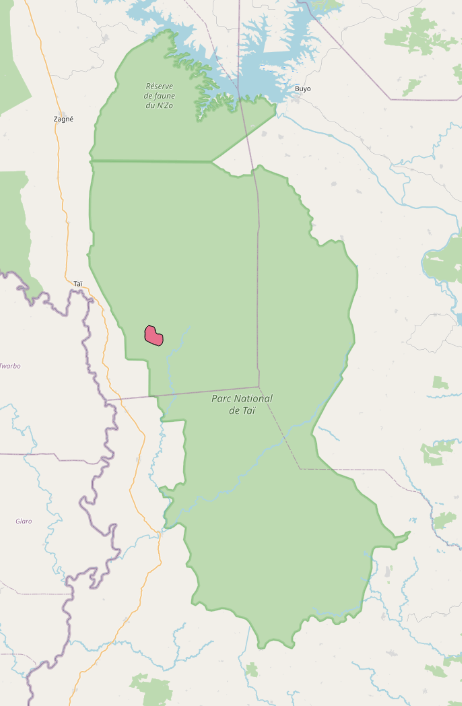
\includegraphics[width=0.43\textwidth]{studyarea-map.png}
\caption{Study area where study of \citet{howeetal} was conducted. \label{fig:map}}
\vspace{-25pt}
\end{wrapfigure}

Using the duiker study described by \citet{howeetal}, this practical helps to design a camera trap distance sampling survey in terms of intensity and spatial arrangement, as well as considering the potential precision we would need when designing a long-term monitoring program. We start by taking a look at the study area in Côte d’Ivoire, where the cameras were deployed according to a systematic grid design with a random start and a 1km spacing between sampling locations.

Maxwell’s duikers were sampled for about 12 weeks using Bushnell camera traps (Model 119576C that gave a horizontal angle of view of 42°) mounted at an orientation of 0° and a height of 0.7–1.0m, and set to high sensitivity. We will treat the survey of \cite{howeetal} as a preliminary study and use the estimates from that study to help inform the design of subsequent surveys. Note that ideally your camera traps should have similar characteristics to those used in the previous study, otherwise you will need to account for that during your design process. Similarly, deploying your cameras with a different orientation or a different height would influence the detectability of your target species of Maxwell’s duikers.

\section{Considerations for a long-term monitoring program}

Assume that we would like to design a long-term monitoring program for Maxwell’s duikers in Tai NP to assess the effectiveness of our work on sustainable conservation management of this population.  As s a first step we can investigate the precision and required effort associated with these planned monitoring surveys relative to the:
\begin{itemize}
	\item cumulative change to the duiker population over the duration of the monitoring, 
	\item number of annual surveys,
	\item power to detect change ($1-\beta$, where $\beta$ is the missed change or type II error) and
	\item false-change error ($\alpha$ level or type I error).
\end{itemize}

To do this we use the equations in \citet{gerrodette1987}. We assume that precision expressed in terms of the coefficient of variation (CV) is a constant over abundance, i.e., it is independent of abundance and thus would remain unchanged by an increase or decrease in abundance, which is frequently assumed for distance sampling surveys. Then equation 10 in \citet{gerrodette1987} allows one to investigate the relationship between these various parameters. For example, if we would like at least 80\% power to detect change in our monitoring program with annual surveys, we set the false-change error ($\alpha$ level) to 20\%, are expecting a 30\% overall increase in the population (based on our assessment of the amount of law enforcement planned and the reproductive capacity of this species) over the course of 15 years of the monitoring program, then this would require a CV of at least 15\%. Given this level of required precision we can then apply a formula to estimate the number of sampling locations that would be required to achieve that precision. 

\section{Effort needed for desired precision}

Maxwell’s duikers sleep or rest for most of each night, so \citet{howeetal}  recorded 11,180 distances from 6:30:00 to 17:59:59 using a 2 second time step during that interval. In the final analysis after truncation of the data 10,284 observations remained giving an average encounter rate of a $3.27 \mbox{x}10^{-4}$ duikers observed per 2 second time interval. Using these data collected at 21 sampling locations a CV of  40\% precision was achieved during this study (here we take a conservative approach and use the estimate of precision derived using bootstrapping rather than the smaller analytical estimate of the CV, which was 27\%). We can estimate how many sampling locations might be needed if we wanted to achieve the level of precision required by our monitoring program when estimating duiker density (CV=15\%). To do this we use the formula for point transect sampling provided by \citet{Bucklandbook}:

\begin{equation}
K_{target}=\frac{K_{pilot}{\mbox{cv}_{pilot}(\hat{D})^{2}}}{{\left\{\mbox{cv}_{target}(\hat{D})\right\}^{2}}}
\end{equation}

where
\begin{itemize}
	\item $K_{pilot}$ number of points in pilot study, 
	\item $\textsf{cv}(\hat{D})$ coefficient of variation from pilot study and
	\item $\textsf{cv}_{target}(\hat{D})$ desired (target) coefficient of variation
\end{itemize}

Given $K_{pilot}$ = 21 and $cv_{pilot}$ = 0.40 from \citet{howeetal} and our $cv_{target}$ of 0.15 we estimate that $K_{target}$ ~ 149 locations. Contrast this estimate of necessary stations for duikers with those and of \cite{cappelle_estimating_2021} for a ~90 day camera deployment (Fig. 5a).

\section{Spatial arrangement of camera stations}

Having computed the necessary amount of sampling effort ($K_{target}$ = 149) to achieve the coefficient of variation to have at least 80\% power to detect a 30\% increase in the population during the 15-year monitoring program for Maxwell’s duikers, the next component of survey design is placement of cameras upon the landscape. \citet{laguardia_assessing_2021} and others advocate a systematic arrangement of sampling stations across a study area.

We will use the survey design feature of Distance for Windows to systematically place the desired number of stations throughout the study area. A Distance project called \emph{Duiker Design}, which has been compressed into a “zip” file, has been set up for this part of the design exercise. Open Distance and extracting the project from the zip file by selecting \textbf{File > Open} project from the menu. Under \textbf{Files of type}, choose \emph{‘Zip archive files (*.zip)’}. Navigate to the folder where you have stored \emph{Duiker Design.zip} and select it. Select a folder to extract the project into and then click OK. Distance will extract the zip archive to the project file \emph{Duiker Design.dst} and the data folder \emph{Duiker Design.dat}, and will then open the project. Next time you want to open the project, you should open the project file \emph{Duiker Design.dst}.  Take a look at the Appendix to this exercise to see how to set up a geographic Distance project for survey design purposes.

Now let’s create a designs for systematically laying out a point grid with a random start that can be used to locate the cameras for this survey. Click on the \textbf{Designs} tab of the \textbf{Project Browser} and then the \textbf{New Design} button (or \textbf{Designs > New Design…} from the menu). Rename your "New Design" something like "Duiker Design 330m" and then click the \textbf{Show Details} button to open the \textbf{Design Details} window (or \textbf{Designs > Design Details…} from the menu). Select the “Point” \textbf{Sampler} and set the design \textbf{Class} to ‘Systematic Grid Sampling’. Click the \textbf{Properties} button to set the following properties for this design:

\begin{itemize}
	\item On the General Properties tab under \textbf{Stratum layer}, the Study area layer should be selected. Under \textbf{Design coordinate system}, the third option is the default to use the previously set up projection.
	\item In the \textbf{Effort Allocation} tab, under \textbf{Edge Sampling} select the “Minus” option. In the \textbf{Allocation by stratum} section leave the \textbf{Point Spacing Units} as “Meter”. Make sure the \textbf{Update effort in real time} check box is ticked. As there is only one survey stratum the ‘Same effort for all strata’ check box is ticked by default and disabled. Click the \textbf{Systematic point grid spacing} radio button. Enter a value of 330 in the Side field and leave the Angle value as zero, as this orientates the point grid in an east-west direction which simplifies field logistics. The Effort is approximated as 161 points and the eventual total number of locations depends on the shape of the survey region, but this should at least give you some indication of what to expect. 
	\item In the \textbf{Sampler} tab, select “Meter” for the line sampler width units. Set the Width to 15 to reflect the limited field of view of the camera.
	\item In the \textbf{Coverage Probability} tab, click on \textbf{Assume even}, as this is a reasonable assumption for this design, so you do not need to check that the coverage probability is even using simulations.
	\item Click \textbf{OK} to close the \textbf{Design Properties} window and return to the design details.
\end{itemize}

Click the \textbf{Run} button on the Design Details window. A window pops up offering you two choices: (1) Calculate coverage probability statistics, and (2) Generate a new survey.  Choose the second option, and give the new Survey a useful name like “SGS330m" and the new layer the same name. Then click OK. A \textbf{Survey Details} window opens, and the status bar at the top of the Distance window says "Running Survey". The software creates a randomly located point grid based on the design. When it is finished, the \textbf{Survey Details Results} tab opens, and you can review some statistics about the new survey. \emph{How many points were generated and how close is this to the approximated total survey effort?}

Click the \textbf{Next>} button to see a map of the point grid. Click \textbf{Next>} again to see a list of the points, with coordinates for each. You could, for example, use this to make a survey plan to take into the field. To copy this text to another file, press the \textbf{Copy current window} button, 4th from the left on the top toolbar. You can also copy the map of grid points by displaying the map and pressing the copy button, or choosing the menu item \textbf{Survey – Results > Copy Map to Clipboard} (another alternative is to open the shapefile in GIS software and to label the point transects there with the labels corresponding to appropriately labelled coordinates you enter into your GPS unit).

Click on \textbf{[X]} to close the \textbf{Survey Details} window, and click on the \textbf{Surveys} tab of the project browser. You can see that your new survey has been added there. If you select it and click the \textbf{Show Details} button (3rd from left after the word \textbf{Survey}) you get back to the \textbf{Survey Details} window \textbf{Results} tab. Click on the \textbf{Inputs} tab and then \textbf{Properties ...} button. Under Data Layers, you can see that the new Sample data layer \textbf{"SGS330m"} has been entered as the lowest sample layer. Close the \textbf{Survey Properties} and \textbf{Survey Details} windows, and click on the \textbf{Data} tab of the Project Browser. You can see that the new sample data layer "SGS330m" has been added below the "Study area" data layer. You can repeat the process by creating new \emph{‘Systematic Grid Sampling’} designs with a different grid spacing. In the same way as before generate survey plans from these designs. 

\section{Additional questions}

\begin{enumerate}
 	\item Repeat the survey design process by creating new \emph{‘Systematic Grid Sampling’} designs with a different grid spacing. In the same way as before generate survey plans from these designs.
 \item Open the Excel spreadsheet “Power Precision Effort Calculations” (see Practical 3-Tuesday folder on website). Take a look at the “Power vs Precision” sheet to see how the estimates of precision change when you change any one of the other parameters (cumulative population change (R), number of annual surveys (S), power to detect change ($1-\beta$), false-change error ($\alpha$)). What precision and effort is needed to achieve 90\% power if the overall decline is 20\% (in both cases leaving the other parameters as they were in the initial scenario)? Examine other scenarios.
\item In the Excel spreadsheet “Power Precision Effort Calculations” take a look at the “Precision vs Effort” sheet to see how the survey effort expressed as number of sampling locations ($K_{target}$) changes with different levels of target precision ($cv_{target}$). 
\end{enumerate}


\printbibliography

\section{Appendix: Setting up a survey design project in Distance}

To set up a geographic project in Distance for the purposes of creating survey designs and generating survey plans, you will need the shape file of you study area, called say “Duikers” and follow these steps:

\begin{enumerate}
	\item Open the Distance software.
	\item Select \textbf{File -> New project...} to create a new project.
	\item When the \textbf{New Project Setup Wizard} pops up select the 2nd \emph{'Design a new survey or simulation'} option and click on \textbf{Next}. 
	\item Select the \emph{'Proceed to Shape Import Wizard'} option and click on \textbf{Finish}. Click on \textbf{Next} gain to get past the introductory screen.
	\item Leave the default ‘Study area’ option as your destination data layer. Browse to the Data folder for this exercise and select the Duikers.shp shapefile and click on \textbf{Next}. 
	\item Allow Distance to \emph{'Copy shapefile to distance project folder'} and check \emph{'Use the coordinate system as the project default'} in this case (the shapefile for this study area is in the geographic coordinate system 'WGS 1984' and click on \textbf{Next}. [HINT: If you project your shapefiles before you use them to generate designs using the Distance software, then this can simplify matters and speeds up calculations.]
	\item On the next screen uncheck \emph{'Use the same projection as the shapefile'} and in the section on \textbf{Map and geographic calculations} set the \textbf{Projection of the map data} to \emph{‘Transverse Mercator’} and the \textbf{Map units} to \emph{‘Meters’}. Click on the \textbf{Parameters…} to set the \textbf{Projection Paramaters} to UTM zone 29N as shown below, which is appropriate for this survey area in Tai National Park. Click on \textbf{OK} when you have entered the values for the \textbf{Projection parameters} and the \textbf{Finish} back on the main screen.

\begin{center}
\begin{figure}[H]
	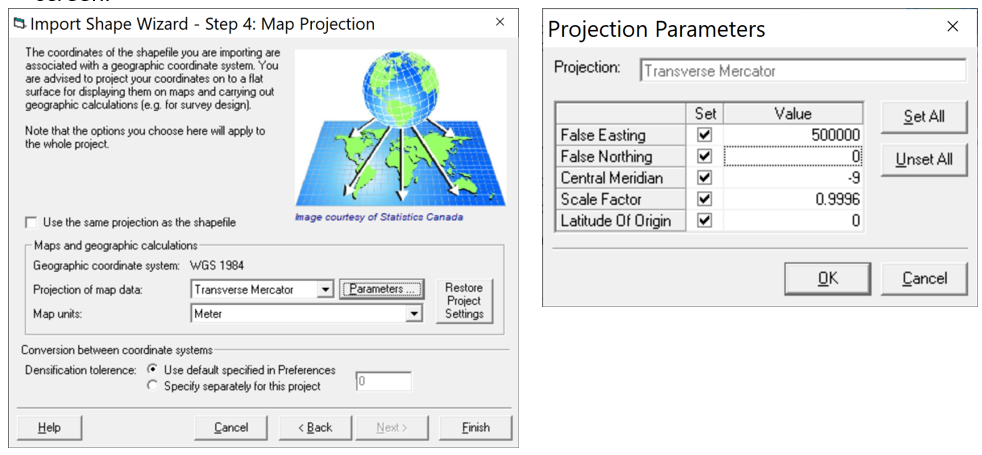
\includegraphics[width=0.8\textwidth]{design-screengrab.PNG}
	\caption{Projection parameter specification when importing shapefiles.}
\end{figure}
\end{center}

	\item When the \emph{‘Create coverage grid’} dialogue box pops up select \textbf{Yes} (a coverage grid is needed to investigate design properties, which we will not be doing here mainly because a systematic grid design with a random start is straightforward with good design properties, such as even spatial coverage and achieving the same sampling intensity throughout the survey area). In the subsequent \textbf{Create New Layer} dialogue box type Grid1000 as your \textbf{Layer name} and retain the remainder of the default options before clicking \textbf{OK}. Click on \textbf{No} in this instance when asked \emph{‘Would you like to import another shapefile?’} (If you were designing a stratified design then you would import a shapefile with your strata at this point.)
	\item Select \textbf{File > Project properties...} and click on the \textbf{Geographic} tab to check that the \textbf{Default coordinate system} is ‘WGS 1984’ and that the \textbf{Map and geographic calculations} are set to UTM 29N. If under Data Layers you right-click on the \textbf{Study Area} and the \textbf{Data Layer Properties…} then on the \textbf{Geographic} tab you should see that the coordinate system is ‘WGS 1984’.
 \item To take a look at the survey region and coverage grid within Distance create a new map in the \textbf{Maps} tab by clicking on the \textbf{New Map} button (or selecting \textbf{Maps > New Map} from the menu). Add the layers Study Area and Grid1000 to the map by clicking on the \textbf{Add Layer to Map} button (or selecting \textbf{Map > Add Layer} from the menu).
\end{enumerate}

%	\item What is the consequence of using bootstrap estimates of uncertainty compared to analytical measures of uncertainty?
%\ifsolutionthenelse{%
%	\begin{tcolorbox}[colback=green!5!white, colframe=green!60!black, title=Differences in $\hat{P}$]
%		Confidence interval bounds widen from (10.4, 32.5) analytical to (8.0, 35.8) bootstrap. Your bootstrap confidence interval bounds will differ from these because of the stochasticity of the bootstrap.
%		\end{tcolorbox}
%}
%{
%}

\end{document}